\subsubsection{Optimization}
\label{sec:optimization}
From the above discussion, one can clearly see that it is
advantageous to split these signal regions so that the dominant
backgrounds in each region may be targeted individually.  Furthermore,
note that while the 1 SFOS region contains more of the signal than the
0 and 2 SFOS regions, it is the 0 SFOS region which is most likely to
have the best sensitivity due to the smaller background contribution.
In \sec\ref{sec:signal_regions} it was already shown
that a selection was chosen based on an optimization procedure
designed to further reduce the background with respect to the 
signal region. The details of the optimization are presented
here.

Within each signal region it may be that we can further reduce the 
background with respect to the signal region. 
By restricting to a region of phase space which removes a larger
fraction of background than it does the signal, we can 
increase the signal prediction with respect to the background.
The ratio of events which pass a selection with respect
to the original number of events is referred to as the 
efficiency.
Thus, we refer to this as choosing a selection threshold where 
the signal efficiency is larger than the background efficiency.
Because the background composition in the 0 SFOS region
is so different from the 1 and 2 SFOS regions, it is likely that
the selection which does this will also differ between them. 
And even though the
1 and 2 SFOS regions are reasonably similar, we should not rule out
the possibility that they also have a uniquely optimal selection.
Based on heuristic arguments, a list of reasonable physical
quantities to restrict were considered. 
Also, because the predicted amount of signal is so precious,
the signal efficiency should be kept as close to unity as possible.
Consider the following selection choices using the quantities defined
earlier:
%Do I need to add more plots here???
\begin{itemize}
\item Lepton $P_{T}$:  Require that exactly three leptons passing tight object quality requirements have a $P_{T} > X$.
\item Missing $E_{T}$:  Require that $\MET > X$.
\item $\Delta\varphi(lll,\MET)$:  Require that $\Delta\varphi(lll,\MET) = \cos^{-1}\frac{ \overrightarrow{p_{T}^{lll}}\cdot\overrightarrow{\MET} }{ p_{T}^{lll}\MET } > X$.
\item Jet Veto: Require that $N_{Jet} \leq X$.
\item b-Jet Veto: Require that $N_{b-Jet} \leq X$.
%\item Z Veto: Require that $m_{ll}$ does not fall in the region $m_{Z}-m_{min} < m_{ll} < m_{Z}-m_{max}$ where $m_Z = 91.1876$~GeV and where $m_{min}$ are $m_{max}$ are the boundaries of the \z-window with which to veto.  For the 1 and 2 SFOS regions the pairs used to construct the $m_{ll}$ are SFOS pairs of either electrons or muons.  In the 0 SFOS region there are no SFOS pairs by definition but there is still a \z-peak in the same-sign di-electron mass spectrum due to charge mis-id. Thus, in the 0 SFOS region we consider instead
\item Three Lepton $m_{T}$: Require that $m_{T}^{lll} > X$
%\item Same-flavor mass: Consider cuts on $m_{SF} > m_{min}$ and/or $m_{SF} < m_{max}$ where $m_{SF}$ is the invariant mass of same-flavor pairs (with no requirement on the sign) %what about this one?
\end{itemize}

\begin{figure}[ht!]
\centering
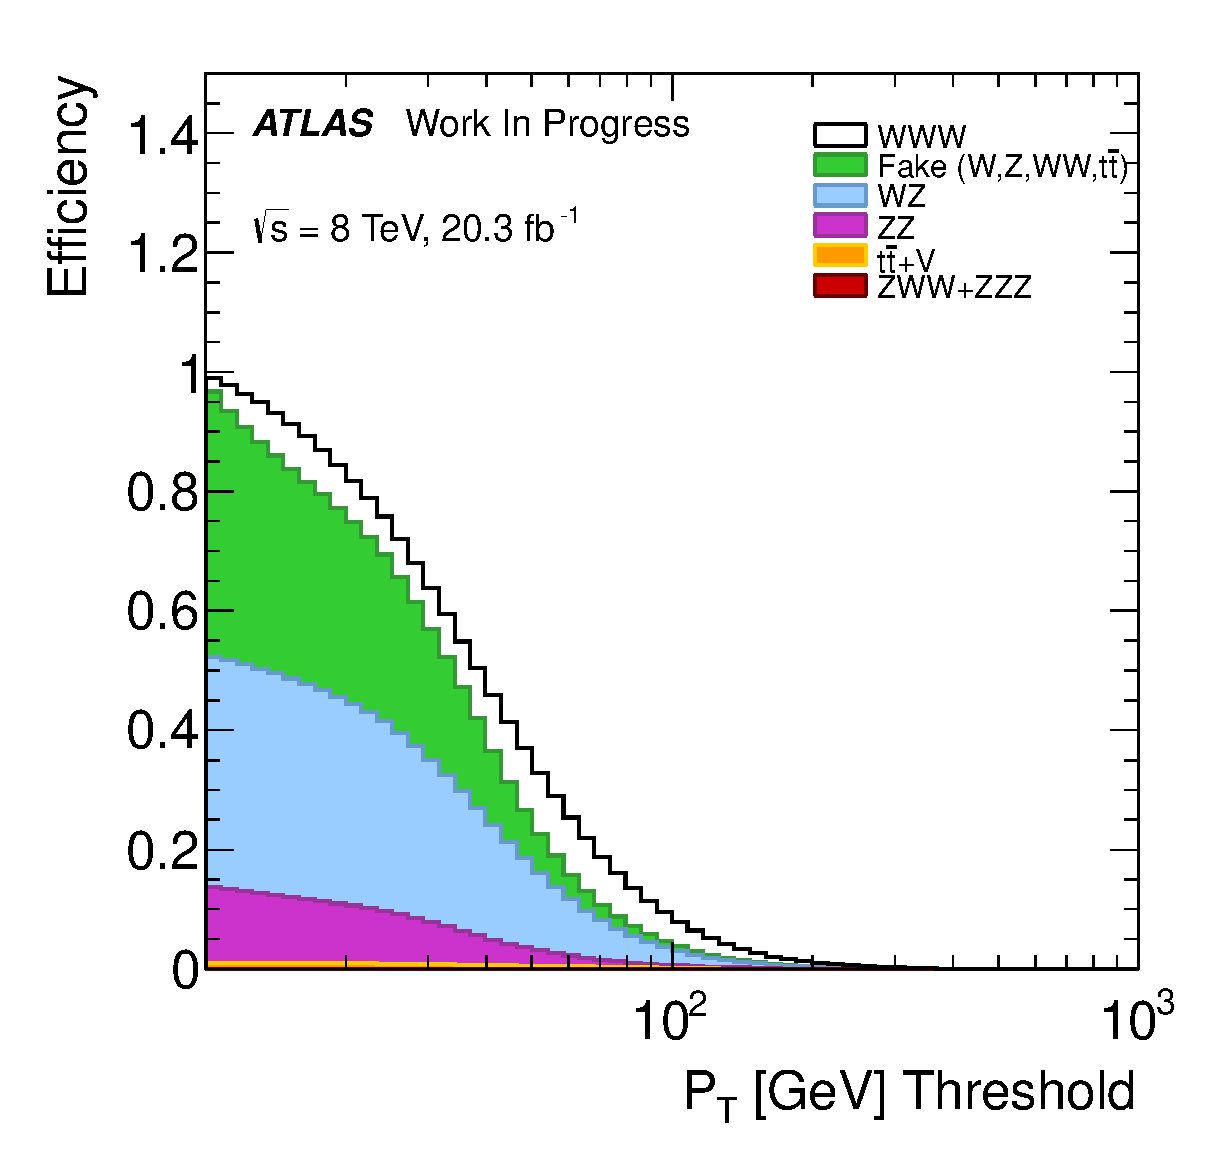
\includegraphics[width=0.3\columnwidth]{figures/optimization/SignalRegions_0p5mmZ0_Preselection_Efficiencies/AllLeptonPt_Cumulative.eps}
\includegraphics[width=0.3\columnwidth]{figures/optimization/SignalRegions_0p5mmZ0_Preselection_Efficiencies/MET_Et_STVF_Cumulative.eps}
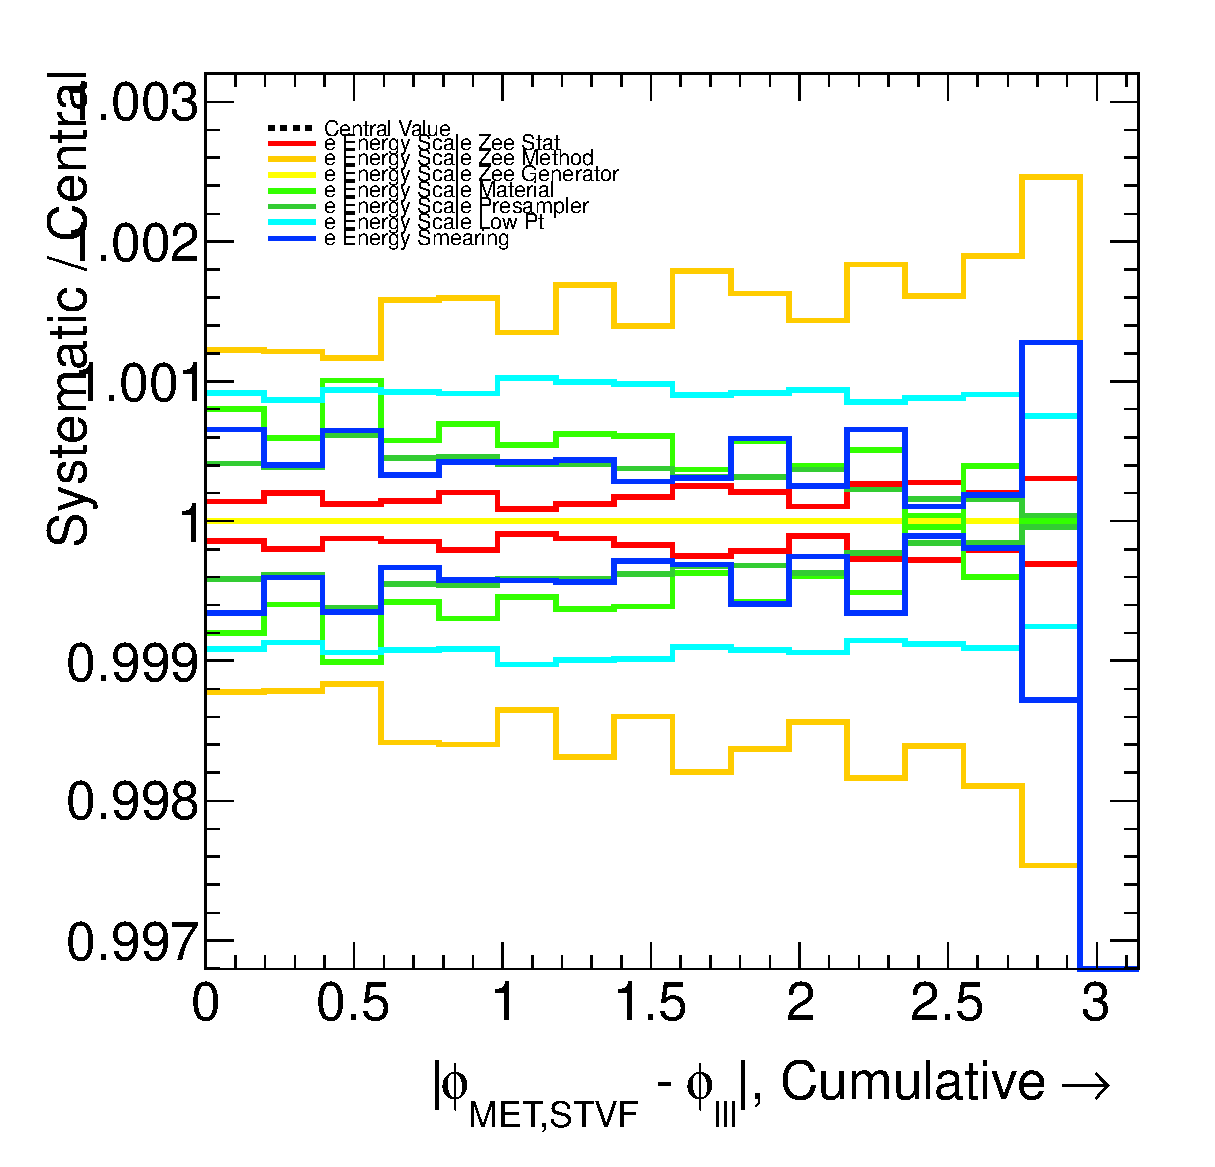
\includegraphics[width=0.3\columnwidth]{figures/optimization/SignalRegions_0p5mmZ0_Preselection_Efficiencies/DeltaPhiMETSTVF123_Abs_Cumulative.eps}
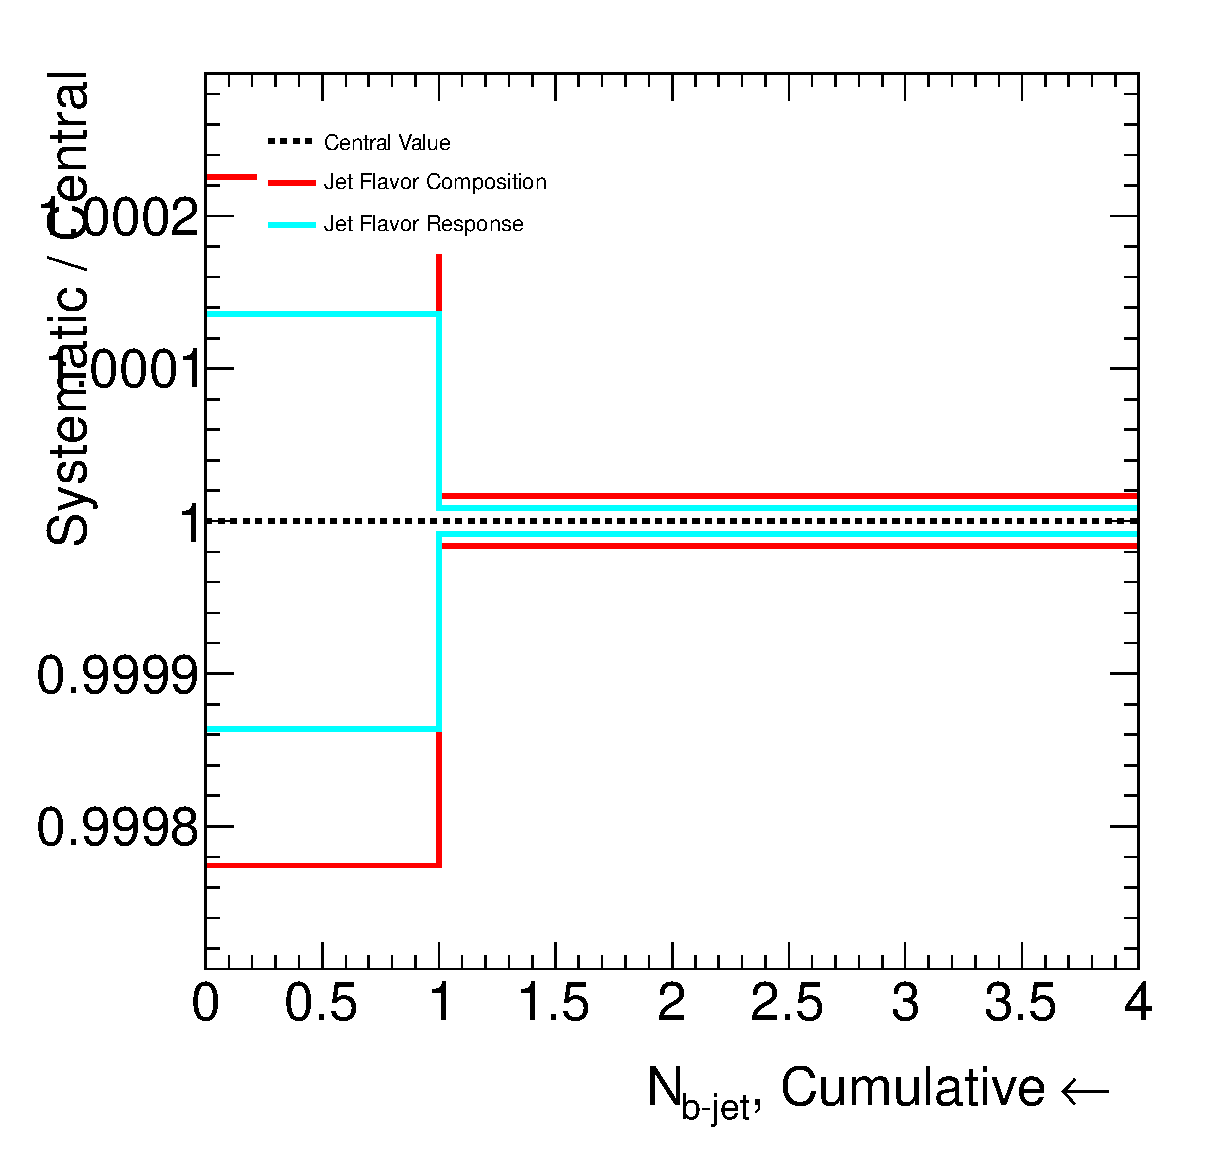
\includegraphics[width=0.3\columnwidth]{figures/optimization/SignalRegions_0p5mmZ0_Preselection_Efficiencies/NBTaggedJets_LeftCumulative.eps}
\includegraphics[width=0.3\columnwidth]{figures/optimization/SignalRegions_0p5mmZ0_Preselection_Efficiencies/NJets_LeftCumulative.eps}
\includegraphics[width=0.3\columnwidth]{figures/optimization/SignalRegions_0p5mmZ0_Preselection_Efficiencies/ThreeLeptonMt_Cumulative.eps}
%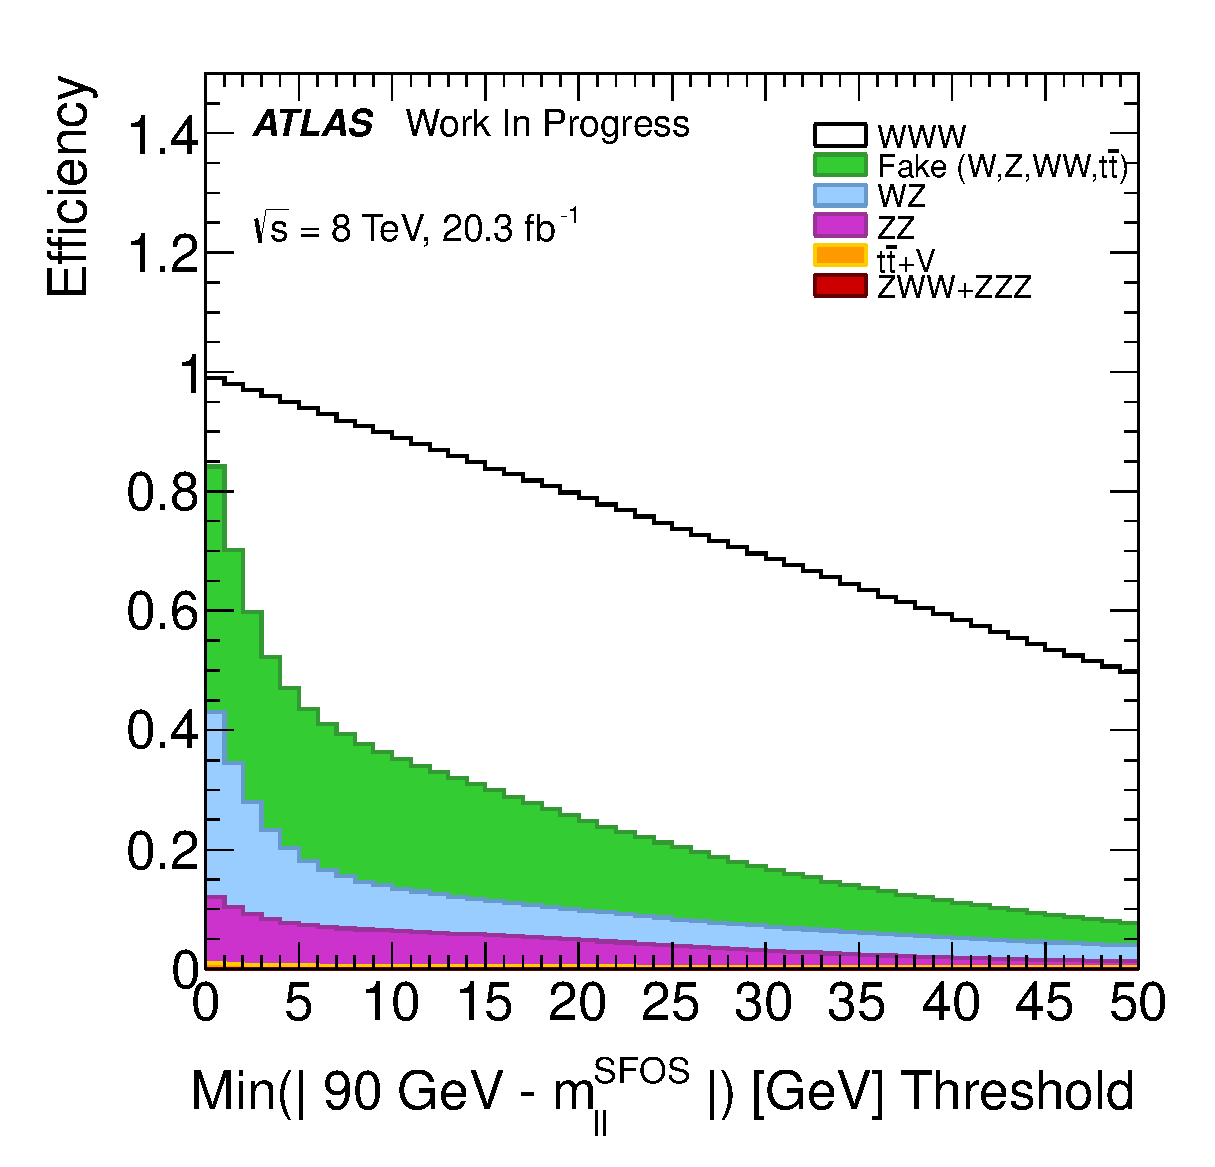
\includegraphics[scale=0.25]{figures/optimization/SignalRegions_0p5mmZ0_Preselection_Efficiencies/ZWindow_Cumulative.eps}
\caption{Signal and background efficiencies as a function of various cuts when starting from event pre-selection.}
\label{fig:optimization_efficiencies_preselection}
\end{figure}



\begin{figure}[ht!]
\centering
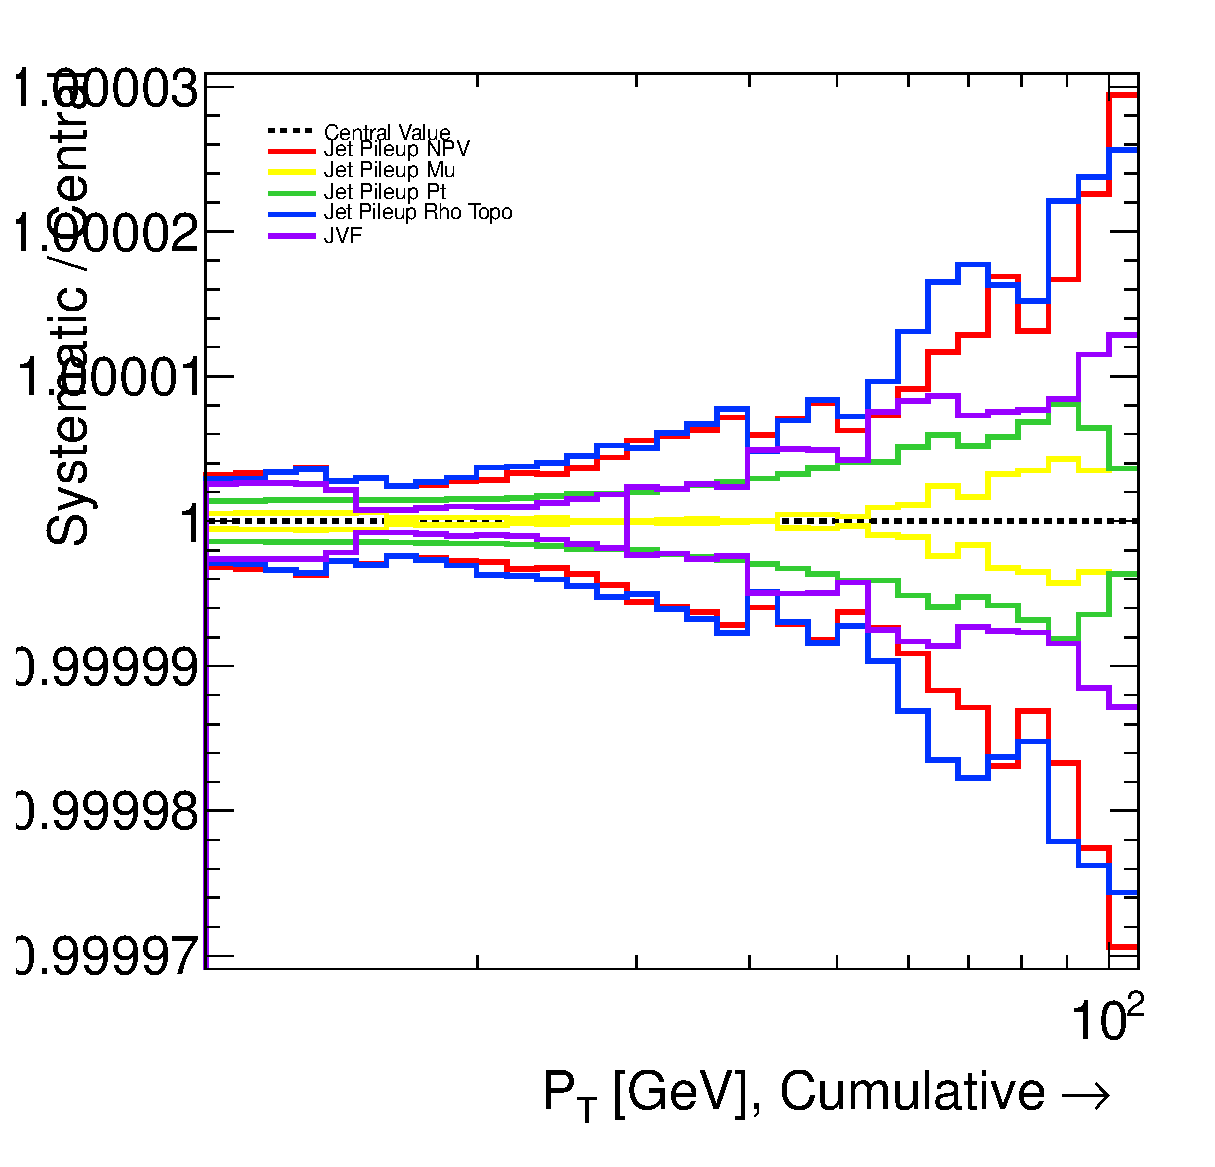
\includegraphics[width=0.3\columnwidth]{figures/optimization/SignalRegionsPreselection_0SFOS_Efficiencies/AllLeptonPt_Cumulative.eps}
\includegraphics[width=0.3\columnwidth]{figures/optimization/SignalRegionsPreselection_0SFOS_Efficiencies/MET_Et_STVF_Cumulative.eps}
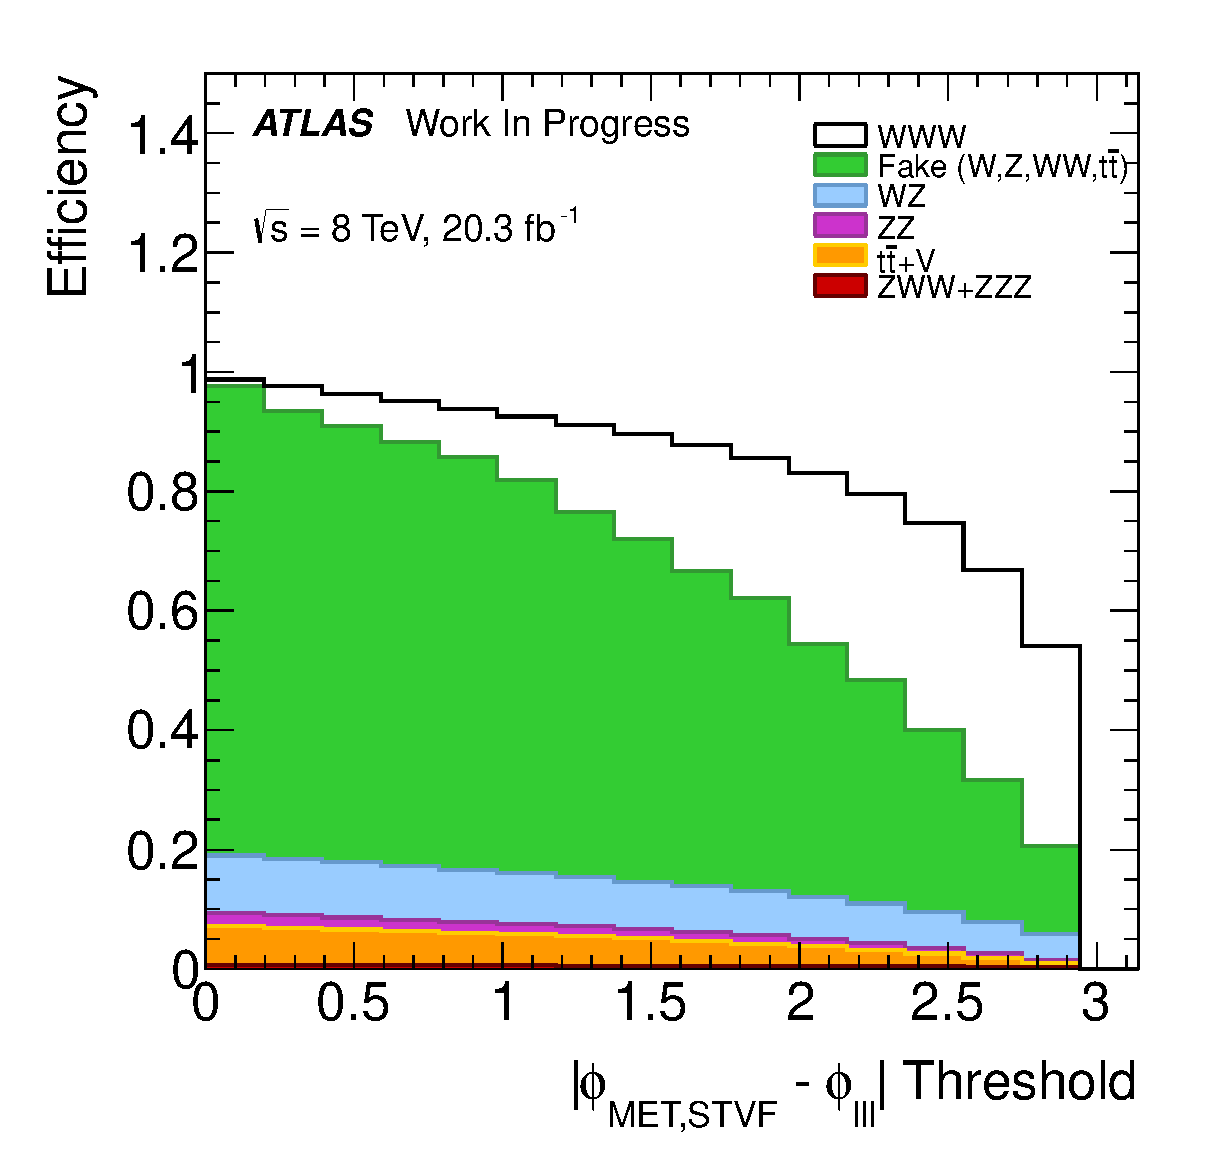
\includegraphics[width=0.3\columnwidth]{figures/optimization/SignalRegionsPreselection_0SFOS_Efficiencies/DeltaPhiMETSTVF123_Abs_Cumulative.eps}
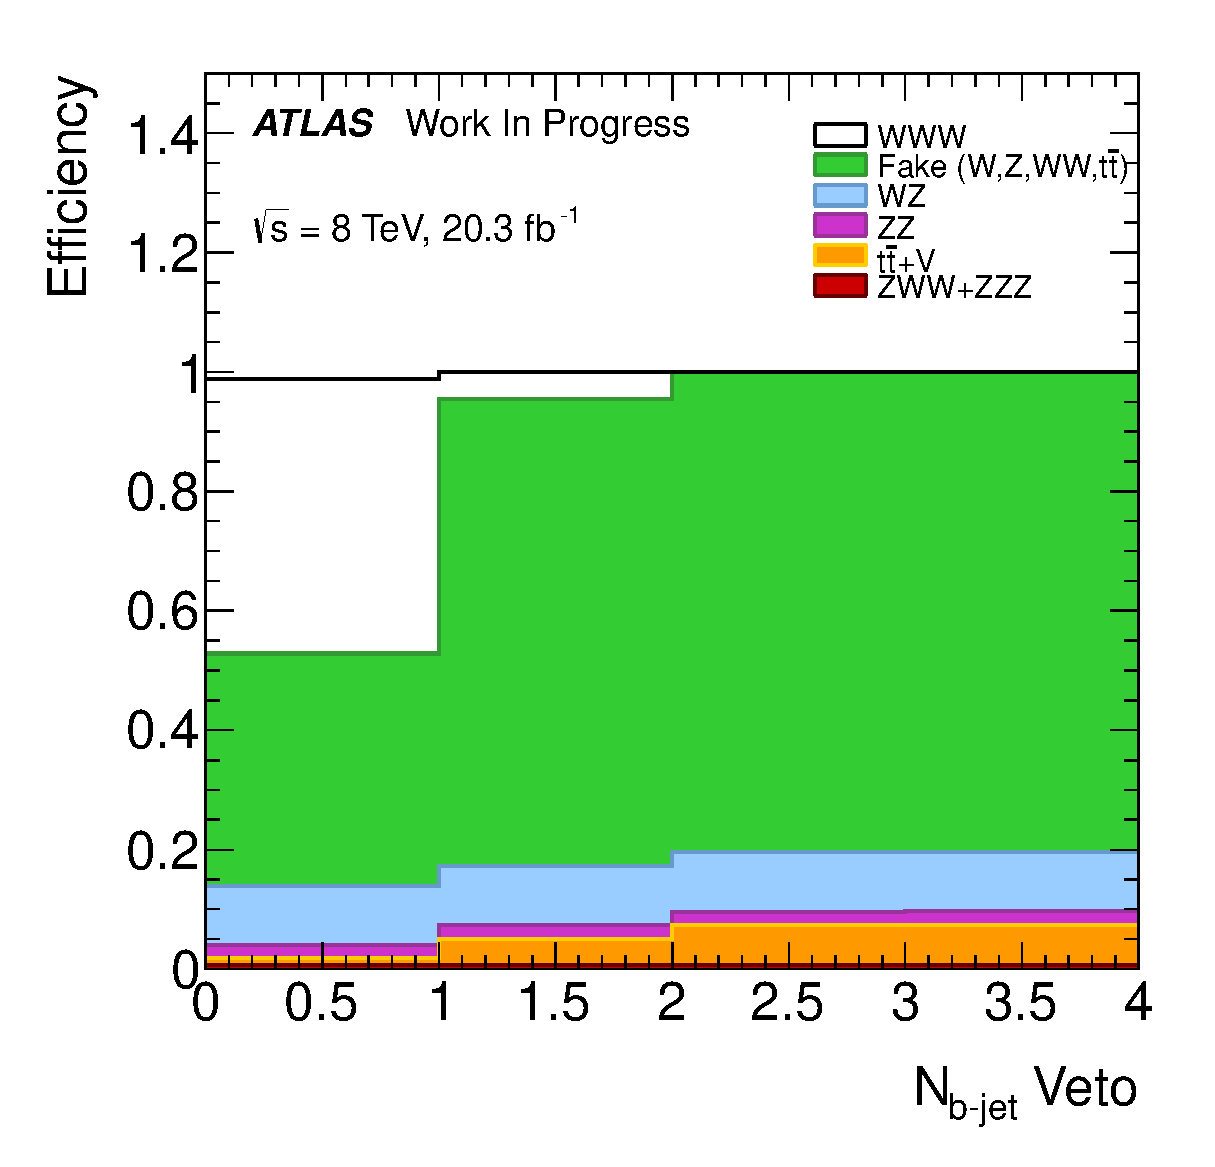
\includegraphics[width=0.3\columnwidth]{figures/optimization/SignalRegionsPreselection_0SFOS_Efficiencies/NBTaggedJets_LeftCumulative.eps}
\includegraphics[width=0.3\columnwidth]{figures/optimization/SignalRegionsPreselection_0SFOS_Efficiencies/NJets_LeftCumulative.eps}
\includegraphics[width=0.3\columnwidth]{figures/optimization/SignalRegionsPreselection_0SFOS_Efficiencies/ThreeLeptonMt_Cumulative.eps}
%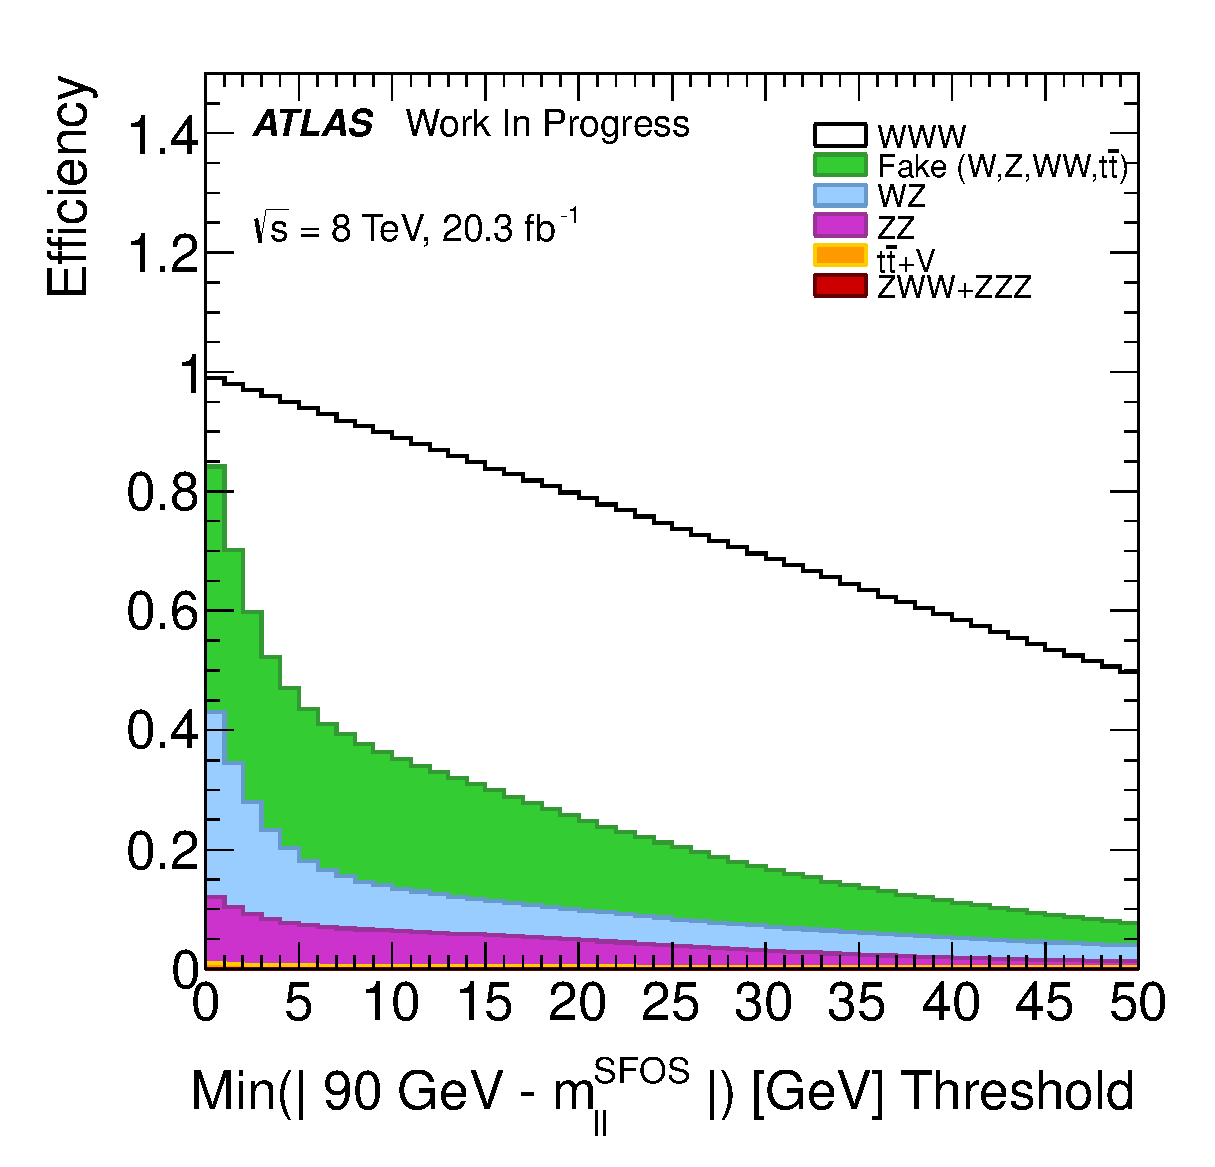
\includegraphics[scale=0.25]{figures/optimization/SignalRegions_0p5mmZ0_Preselection_Efficiencies/ZWindow_Cumulative.eps}
\caption{Signal and background efficiencies as a function of various cuts when starting from event pre-selection + 0 SFOS lepton pairs.}
\label{fig:optimization_efficiencies_0sfos}
\end{figure}

We can plot the efficiency for the signal as well as the background
as a function of the threshold, $X$, for each of these quantities. 
The efficiencies are shown starting 
in the pre-selection region in 
\fig\ref{fig:optimization_efficiencies_preselection} 
(which has a similar background composition to the 1 and 2 SFOS regions)
and in the pre-selection + 0 SFOS region
in \fig\ref{fig:optimization_efficiencies_0sfos}.
Clearly, the shape of the efficiencies between the signal and
background is not always the same, which means that we have some
power to reduce the background with respect to the signal.
Furthermore, these shapes are not the same in the pre-selection 
+ 0 SFOS region as they are in just the pre-selection region.
For instance, in the 0 SFOS region, the shape of the efficiencies
for signal and background are very similar as a function
of the \MET~threshold, but in the pre-selection stage they are
very different, with the background efficiency dropping much
more rapidly than the signal efficiency. This suggests that
a cut on the \MET~distribution could be very useful 
in the 1 and 2 SFOS regions but not in the 0 SFOS region.
Something similar may be true for a cut on $m_{T}^{lll}$.
On the other hand, a cut on \deltaphi~ could prove useful in all 
signal regions. The lepton \pt~is frequently used as a useful discriminant
but in this case it seems to rapidly remove the signal at about the
same rate as the background, so a tighter cut on the lepton \pt~
is likely to prove to be not useful. Cuts on \njet~seem to remove a lot of 
the signal but cut tighter on the background in the pre-selection
+ 0 SFOS region, which could prove useful.  Most impressive is 
the cut on \nbjet, which leaves the signal efficiency at almost exactly
one, while having a large impact on the pre-selection + 0 SFOS region
where the fake contribution is large.

This type of heuristic study  can be used to obtain insight into
the distributions that are useful for discriminating 
between signal and background.  But using these distributions
alone to determine a final selection is a little haphazard.
For one, they do not tell us the impact that cutting on multiple
distributions will have.  These distributions are likely to be 
at least partially correlated, so that cutting on one distribution might
enhance or deflate the impact of another cut. 
And two, it is not at all clear from these distributions
what is the best choice of cuts. We need a metric that will
allow us to make decisions about which cuts to choose.
The metric to use should be one that is 
related to the final prediction after all selection cuts are applied.
Thus, the metric cannot be used to make a decision about each 
cut individually, but instead about some combination of cuts.

To deal with the issues mentioned above, we 
decided on the final signal region selection using an optimization
procedure. The optimization takes as input a multi-dimensional 
space where each dimension is the selection threshold
for one of the quantities listed above, plus some others not mentioned.
The range of the multi-dimensional space that is 
is restricted so that the 
predicted signal remains finite i.e. non-zero.
At an individual point in this space, the optimization computes
the expected signal and background events after the selection
along with the size of statistical uncertainties
and systematic uncertainties on the model. 
These are then used as input to the measurement extraction framework
described in \sec\ref{} to determine the width of the precision
on the final measurement. 
This width is used as the metric to minimize in the optimization.
By considering a metric like this, we are optimizing directly
the quantity of interest to the final measurement, and taking
into account not just the individual predictions, but also their
uncertainties. This is important because it can more stringently
remove backgrounds that have large uncertainties.

We choose to treat the sample space as being discrete as opposed
to continuous. For some dimensions of the space, such as 
the threshold on \njet, this is manifestly true, as there 
can only be an integer number of observed jets. 
For other dimensions, such as the threshold on the lepton
\pt, these quantities are real valued and thus continuous.
However, looking at \fig\ref{fig:optimization_efficiencies_preselection} 
and \fig\ref{fig:optimization_efficiencies_0sfos}, the shape
of the efficiencies tend to change relatively slowly from bin
to bin. Thus, it should be acceptable to only sample 
discretely as long as they can capture the shape information of 
the efficiencies as they do above. Furthermore, 
this acknowledges the finite  experimental resolution of these 
quantities. For example,
the difference between $\pt > 20~\GeV$ and $\pt > 20.5~\GeV$
should not be taken too seriously because of the effects of limited
track and energy resolution used to derive the muon and electron \pt.
%expand on this? what would be the typical electron and muon resolution here?
Treating the sample space as discrete means that the optimization
function is not smooth and so cannot readily take into account
derivative information to be used for instance 
in some sophisticated minimization algorithm.
Fortunately, the number of points in the sample space after discretizing, 
while large, is small enough that it can be evaluated in its entirety
using a brute force approach. Thus, we choose to evaluate the 
optimization in the restricted and discretized sample space in order
to find an optimal choice for the selection.

%I should redo the optimization for the specific bin sizes and list them

The shape of the optimization can be seen in \fig\ref{fig:optimization}.
\emph{Figures need to be reproduced. Elaborate...} 


\begin{figure}[ht!]
\centering

\includegraphics[width=0.3\columnwidth]{figures/placeholder.eps}

\includegraphics[width=0.3\columnwidth]{figures/placeholder.eps}

\includegraphics[width=0.3\columnwidth]{figures/placeholder.eps}
\caption{Signal Yield vs Measurement Uncertainty for optimized points 
in the 0 SFOS (left), 1 SFOS (middle), and 2 SFOS (right) signal regions.}
\label{fig:optimization}
\end{figure}



\begin{figure}[ht!]
\centering
\includegraphics[width=0.4\columnwidth]{figures/appendix_signal_selection/Nov24Update_FakeSys_KFacSys_LogY_NoRebin/output/jobs/MxM/DataFull_Rates_May13_FakeRatesExactly2Loose_MuonMxMBJetGt0_ElBJetGt0SubtractPC_MxM/PreselectionNov23_15_1SFOS_ChargeAbs1_BVeto85_physics/weight_all/png/MET_Et_histratio.png}
\includegraphics[width=0.4\columnwidth]{figures/appendix_signal_selection/Nov24Update_FakeSys_KFacSys_LogY_NoRebin/output/jobs/MxM/DataFull_Rates_May13_FakeRatesExactly2Loose_MuonMxMBJetGt0_ElBJetGt0SubtractPC_MxM/PreselectionNov23_15_1SFOS_ChargeAbs1_BVeto85_physics/weight_all/png/InvariantMassSFOS_histratio.png}
\includegraphics[width=0.4\columnwidth]{figures/appendix_signal_selection/Nov24Update_FakeSys_KFacSys_LogY_NoRebin/output/jobs/MxM/DataFull_Rates_May13_FakeRatesExactly2Loose_MuonMxMBJetGt0_ElBJetGt0SubtractPC_MxM/PreselectionNov23_15_2SFOS_ChargeAbs1_BVeto85_physics/weight_all/png/MET_Et_histratio.png}
\includegraphics[width=0.4\columnwidth]{figures/appendix_signal_selection/Nov24Update_FakeSys_KFacSys_LogY_NoRebin/output/jobs/MxM/DataFull_Rates_May13_FakeRatesExactly2Loose_MuonMxMBJetGt0_ElBJetGt0SubtractPC_MxM/PreselectionNov23_15_2SFOS_ChargeAbs1_BVeto85_physics/weight_all/png/InvariantMassSFOS_histratio.png}
\caption{Plots of the \MET (left) and $m_{\textrm{SFOS}}$ (right) distributions 
in the 1 SFOS (top) and 2 SFOS (bottom) regions after pre-selection
plus the \bee-veto requirement.}
\label{fig:met_zwindow_optimization}
\end{figure}

The $Z\gamma$ background shows up in the low-shoulder of the \z-peak
in the $m_{\textrm{SFOS}}$ distribution and at low MET. This can be
seen both for the 1 and 2 SFOS regions in \fig\ref{fig:met_zwindow_optimization}.
As a result, the $Z\gamma$ background can be removed either by tuning 
the \z-mass window used in the veto above, or by removing events with low \met.
Thus, the optimization shows that there is some correlation 
between the \z-veto window and the \met~selection threshold. 
In the 1 SFOS region, there is a larger 
contribution from $Z\gamma$ processes than in the 2 SFOS
region.  This process mostly shows up in the low shoulder 
of the \z~ peak. The optimization
prefers removing this $Z\gamma$ contribution by setting an 
asymmetric \z-window in the 1 SFOS
region, with the boundaries being 35~GeV below the \z-pole 
and 20~GeV above and then keeping the \MET cut a little loose, with a 
threshold of $\MET > 45$~GeV.  Meanwhile, in the 2 SFOS region,
the $Z\gamma$ contribution is not as prominent and the 
optimization happens to prefer a symmetric
window of $\pm20$~GeV around the \z-pole.  
The looser \z-veto then allows for a tighter
missing $E_{T}$ cut with a threshold of $\MET > 55$~GeV. 
In the 0 SFOS region there 
are no SFOS pairs by definition,
but there is still a peak in the same-sign electron-electron mass 
distribution due to charge mis-identification.
The optimization prefers a slightly narrower symmetric window 
of $\pm15$~GeV around the \z-mass. 
Further, as already mentioned,
this background turns out 
to have a similar missing $E_{T}$ distribution
as the signal. As a result, cutting on the missing $E_{T}$ in this region 
offers little to no discriminating power
between the signal and background so we have chosen not to apply 
any cut here in order to maximize the signal yield.

